\blindtext
\section{El perceptrón multicapa}
El perceptrón multicapa es una generalización del perceptrón simple de
Rosenblatt, como consecuencia de las limitaciones de éste ante
conjuntos de datos que no son linealmente separables. Lo que se hace
es combinar varios perceptrones en una \textit{red neuronal de
  propagación hacia adelante}, con una estructura de \textit{capas}.

La información fluye de capa en capa en el mismo sentido, desde la
\textit{capa de entrada} donde están los datos sin procesar, hasta la
\textit{capa de salida} dónde se da la clasificación. Cada una de las capas
intermedias, llamadas \textit{capas ocultas}, consta de un conjunto de
neuronas sin conexiones entre ellas, pero totalmente conectadas a las
capas inmediatamente anterior y posterior. Visto como una gráfica, un
\textbf{perceptrón multicapa} (MLP, \textit{Multilayer Perceptron})
es una gráfica $n$-partita dirigida donde $n$ seria el número de
capas.
\begin{figure}[H]
  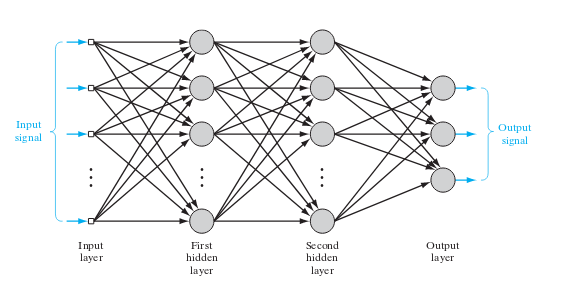
\includegraphics[scale=1.3]{mlp} \centering \caption{Arquitectura de
  un MLP con una capa oculta (Tomado de \url{https://es.wikipedia.org/wiki/Perceptron_multicapa})}
\end{figure}
Cada neurona oculta actua como un \textit{detector de
  características}. Conforme va avanzando el proceso de aprendizaje,
las neuronas ocultas comienzan a ``descubrir'' gradualmente las
características más sobresalientes de los datos de entrenamiento.
Esto se logra a través de una serie de transformaciones no lineales,
dadas por las funciones de activación y pesos específicos de cada
neurona.

Inicialmente, a cada neurona se le asigna un peso aleatorio. Dada la
estructura en capas de la red, es mucho más fácil visualizar y
manipular estos pesos acomodandolos en una matriz $W$, que llamaremos
\textit{matriz de pesos}, donde $W_i$ son los pesos de la $i$-ésima
capa de la red. Entonces, dado un vector de entrada $x$, la primera
capa oculta $h_1$ calcula su valor a partir de $W_1$ y una traslación
$b_1$, que llamamos \textit{sesgo} (en inglés, \textit{bias}), del
siguiente modo:
\begin{equation}
  h_1 = \sigma(W_1x + b_1)
\end{equation}
donde $\sigma$ es una función de activación no lineal y
diferenciable. Así la $i+1$-ésima capa oculta computa su valor como
\begin{equation}
  h_{i+1} = \sigma(W_{i+1}h_i + b_{i+1})
\end{equation}
Por último, la salida, suponiendo que hay $n$ capas ocultas, seria
\begin{equation}
  \hat{y} = \sigma{(W_{n+1}h_n + b_{n+1})}
\end{equation}
donde $\hat{y}$ es el vector de clasificación.

\section{Descenso por el gradiente}
Uno de los puntos clave del aprendizaje de máquina supervisado es
definir una función objetivo que deberá ser optimizada durante el
proceso de aprendizaje. Esta función objetivo usualmente es una
\textbf{función de costo, pérdida o error} que se quiere minimizar.

Definimos la función de costo $J$ como la \textbf{Suma de los errores
  cuadrados} (SSE, \textit{Squared Sum Error}) entre la salida
  calculada y el valor real.
\begin{equation}
  J(w)=1/2n \sum_i (\hat{y}_i - y_i^2)
\end{equation}
donde $w$ es el conjunto de los parámteros de la red, es decir $w :=
\bigcup{W_i, b_i}_{i=1}^{n}$, $n$ el número de capas de la red, y
$y_i$ la $i$-ésima etiqueta de entrenamiento. La principal ventaja de
esta función de error, además de ser lineal es que la función de
costos se vuelve diferenciable.

La no-linealidad de las funciones de activación provoca que no se
garantice la convexidad de las funciones de error más comunes, es
decir, que no existe un método analítico para encontrar el mínimo de
la función de error. El entrenamiento de la red se basa en métodos
iterativos que van reduciendo paulatinamente ese error.

Sabemos que la derivada es útil para minimizar funciones porque, dada
una función $y = f(x)$, nos dice cómo cambiar $x$ para hacer una
pequeña mejora en $y$, en otras palabras $f(x-\varepsilon f'(x)) <
f(x)$ para un $\varepsilon \in \mathbb{R}$ suficientemente
pequeño. Podemos entonces minimizar $f(x)$ al mover a $x$ en pequeños
\textit{pasos} con el signo opuesto de la derivada. A esta técnica se
le conoce como \textbf{descenso por el gradiente}.

La idea detrás del descenso por el gradiente es disminuir el gradiente hasta encontrar
un mínimo (local o global) de la función de costo. En cada iteración, se reduce
un \textit{paso} del gradiente, donde cada \textit{paso} está determinado por
el valor del índice de aprendizaje, así como por la pendiente del gradiente.

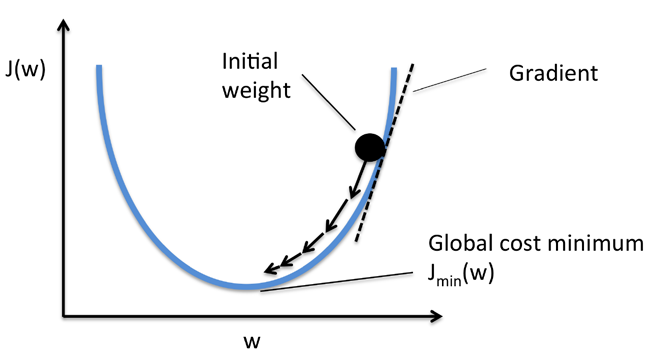
\includegraphics[scale=0.5]{gradient-descent}

Usando el descenso por el gradiente, se pueden actualizar los pesos quitandole un \textit{paso}
al gradiente $\nabla J(w)$ de la función de costos $J(w)$:
\begin{equation}
  w := w + \Delta w
\end{equation}

En donde el cambio de peso $\Delta w$ se define como el gradiente negativo multiplicado
por el índice de aprendizaje $\eta$:
\begin{equation}
  \Delta w := -\eta \Delta J(w)
\end{equation}

Calculamos la derivada parcial de la función de costos SSE con respecto al
j-ésimo peso de la siguiente manera:
\begin{equation*}
\begin{split}
  \frac{\partial J}{\partial w_j} &= \frac{\partial}{\partial w_j}\frac{1}{2}\sum_i (y^{(i)} - \phi(z^{(i)}))^2 \\
  &= \frac{1}{2}\sum_i 2(y^{(i)} - \phi(z^{(i)}))\frac{\partial}{\partial w_j}(y^{(i)} - \phi(z^{(i)}))\\
  &= \sum_i (y^{(i)} - \phi(z^{(i)}))\frac{\partial}{\partial w_j}(y^{(i)} - \phi (z^{(i)}))\\
  &= \sum_i(y^{(i)} - \phi(z^{(i)}))(-x_j^{(i)})\\
  &= -\sum_i(y^{(i)} - \phi(z^{(i)}))x_j^{(i)}
\end{split}
\end{equation*}

Las redes neuronales (ANN, \textit{Artificial Neural Network}) son
modelos complejos que por lo general tienen un alto número de mínimos
locales, volviendo al descenso por el gradiente poco efectivo como
mecanismo de entrenamiento.  Sin embargo, redes altamente eficientes
usualmente son entrenadas utilizando descenso por el gradiente. ¿Cómo
explicar esta aparente contradicción?

Recientemente, evidencia empírica \cite{choromanska} ha dado indicios
de que las ANN tienen la mayoría de sus mínimos locales cerca del
mínimo global.  Esto quiere decir que \textbf{el descenso por el
gradiente funciona ``suficientemente bien''}. Hay otros métodos más
avanzados que son empleados para entrenar ANNs, pero en este trabajo
utilizamos descenso por el gradiente por su simplicidad e
interpetación tan intuitiva.

\section{Retropropagación}
Para utilizar de forma efectiva el descenso por el gradiente, es
necesario una forma eficiente de computar el gradiente de una función
de error. La propagación hacia atrás o retropropagación
(\textit{Backpropagation}) nos permite hacerlo.

Definimos para cada neurona $j$ en la capa $l$ la salida $o^{(l)}_j$ como
\begin{equation}
\label{eqn:def_o}
  o^{(l)}_j = \phi(a^{(l)}_j) = \phi(\sum_{k=1}^n w_{kj}o_k^{(l-1)})
\end{equation}
donde $\phi$ es la función de activación y $a_j^{(l)}$ se refiere a la
suma de los pesos de las salidas de las neuronas de la capa inmediata
anterior. Comunmente, llamamos a $a_j^{(l)}$ la \textit{activación} de
la neurona.

Supongamos ahora que queremos encontrar la derivada parcial de la
función de errir con respecto a $w_{ij}$.
Para encontrar cómo cambia una función de error $J$ cambia con respecto
al peso $w_{ij}$, aplicamos la regla de la cadena:
\begin{equation}
  \frac{\partial J}{\partial w_{ij}} = \frac{\partial J}{\partial o_j^{(l)}}
  \frac{\partial o_j^{(l)}}{\partial a_j^{(l)}} \frac{\partial a_j^{(l)}}{\partial w_{ij}}
\end{equation}

A partir de \ref{eqn:def_o}, podemos ver que
$a_j^{(l)} = \sum_{k=1}^n w_{kj}o_k^{(l-1)}$. Esto implica que
$\frac{\partial a_j^{(l)}}{\partial w_{ij}} = o_i^{(l-1)}$. Definimos entonces
\begin{equation}
  \delta_j^{(l)} = \frac{\partial J}{\partial o_j^{(l)}} \frac{\partial o_j^{(l)}}{a_j^{(l)}}
\end{equation}

Así, tenemos que
\begin{equation}
  \frac{\partial J}{\partial w_{ij}} = \delta_j^{(l)}o_i^{(l-1)}
\end{equation}
Resulta entonces que tenemos una identidad recursiva para
$\delta_j^{(l)}$, llamada la fórmula de la retropropagación
\begin{equation}
  \delta_j^{(l)} = \phi'(a_j^{(l)})\sum_m w_{jm} d_m^{(l+1)}
\end{equation}
donde la suma es sobre las neuronas conectadas a la $j$-ésima neurona
de la capa $l$.

Podemos entonces derivar esta identidad utilizando la regla de la cadena
para escribir $\frac{\partial J}{\partial o_j^{(l)}}$ en términos de
$\frac{\partial J}{\partial a_m^{(l+1)}}$ y $\frac{\partial a_m^{(l+1)}}{\partial o_j^{(l)}}$.

\begin{equation}
\begin{split}
  \delta_j^{(l)} &= \frac{\partial J}{\partial o_j^{(l)}} \frac{\partial o_j^{(l)}}{\partial a_j^{(l)}} \\
  &= \frac{\partial o_j^{(l)}}{\partial a_j^{(l)}} \frac{\partial J}{\partial o_j^{(l)}} \\
  &= \phi' (a_j^{(l)}) \sum_m \frac{\partial J}{\partial o_m^{(l+1)}} \frac{\partial o_m^{(l+1)}}{\partial a_m^{(l+1)}} \frac{\partial a_m^{(l+1)}}{\partial o_j^{(l)}} \\
  &= \phi'(a_j^{(l)}) \sum_m \delta_m^{(l+1)}w_{jm}
\end{split}
\end{equation}

Notemos que esto nos permite computar capas anteriores a $\delta_j$ a
través de las capas posteriores --- de ahí el nombre de retropropagación.
Podemos computar $\delta_j$ directamente, si $j$ es una capa de salida,
así que este proceso eventualmente termina.
